\section{Main results: coverage explains the observed action gain}
All \MainCalls{} planned requests completed, with no schema or transport failures. The audit reconstructs 7,392 context packets and re-scores every raw response. The same-backbone results are identical for the two readers on this formal task; that agreement is not two independent company samples.

\begin{table}[t]
\centering\small\begin{tabular}{lrrr}
\toprule
Context & Complete support & GPT correct & Claude correct \\
\midrule
No context & 0/132 & 132/264 & 132/264 \\
Generic hybrid & 91/132 & 223/264 & 223/264 \\
Structured Markdown & 132/132 & 264/264 & 264/264 \\
GBrain search & 20/132 & 152/264 & 152/264 \\
Specialized coverage & 132/132 & 264/264 & 264/264 \\
GBrain + coverage & 132/132 & 264/264 & 264/264 \\
Full current context & 132/132 & 264/264 & 264/264 \\
\bottomrule
\end{tabular}

\caption{Frozen main study at 2,048 evidence bytes. Complete support is measured on 132 answerable cases; grounded correctness includes those 132 cases and 132 required-withholding cases. Each reader executes 264 requests per row. Full context is an unequal-budget reference.}
\label{tab:main}
\end{table}

\paragraph{Context availability.}
Generic hybrid retrieves complete support for \CompleteGeneric/\MainPositives{} answerable cases (68.9\%); specialized coverage retrieves \CompleteSpecial/\MainPositives{}. Native GBrain search supplies 20/132 under this small allowance, while adding the same coverage layer raises it to 132/132. Structured Markdown also supplies 132/132 without catalog-specific priorities. This last control rules out a claim that a domain ontology or proprietary backend is required at the primary budget.

\begin{figure}[t]
\centering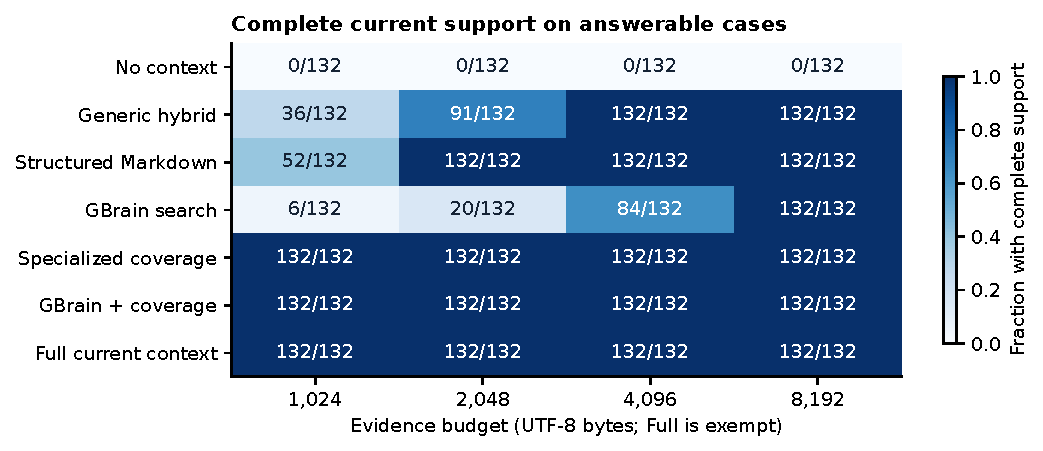
\includegraphics[width=\linewidth]{figures/integrated/retrieval-budget.pdf}
\caption{Retrieval-only budget sweep on the same 132 answerable cases. At 1,024 bytes, specialization preserves complete support while generic diversity often cannot. Generic hybrid closes the gap at 4,096 bytes; native GBrain search does so at 8,192. Reader experiments use 2,048 bytes only; lower-budget recommendation gains are not inferred from this figure.}
\label{fig:budget}
\end{figure}

\paragraph{Grounded decisions.}
Specialized context improves each reader from \GptGenericCorrect/\MainCases{} to \GptSpecialCorrect/\MainCases{} correct decisions (Figure~\ref{fig:reader}). The paired gain is \GptDifference{} percentage points, 95\% interval [\GptLow{},\GptHigh{}]; the Holm-adjusted exact paired sign-test value is $1.22\times10^{-4}$ for each provider. The effect is positive in 15 worlds and zero in 18. Positive recommendation coverage rises 31.1 points, from 68.9\% to 100\%: 41 additional supported recommendations among 132 answerable cases, or 45.1\% more than the 91 produced with Generic. These percentages describe formal eligibility and citations, not a 45.1\% improvement in strategic value.

\begin{figure}[t]
\centering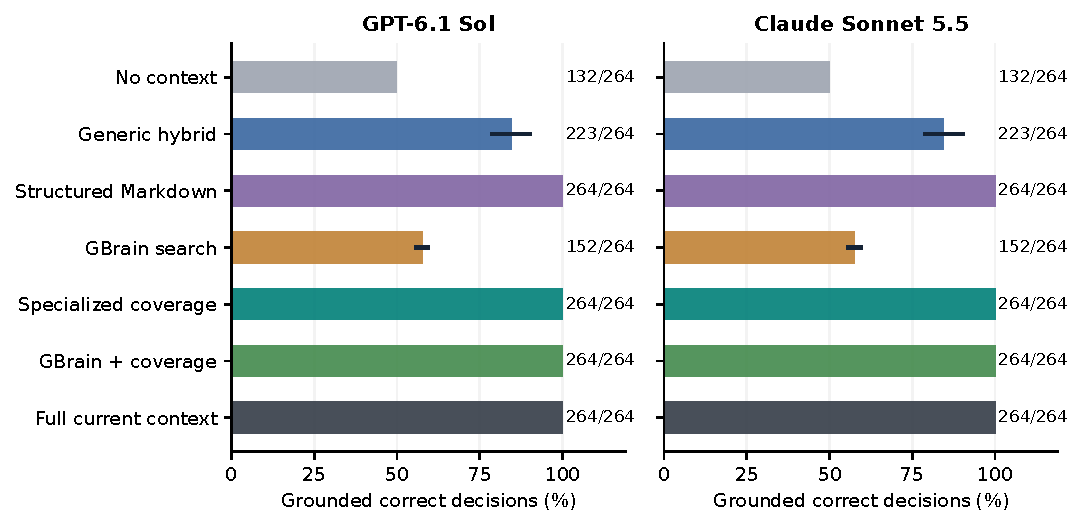
\includegraphics[width=\linewidth]{figures/integrated/reader-quality.pdf}
\caption{Grounded correct decisions with fixed readers. Bars start at zero; lines are 95\% family-stratified world-bootstrap intervals. Several methods reach the fixture ceiling, so their empirical intervals collapse; this does not establish universal perfection.}
\label{fig:reader}
\end{figure}

\begin{figure}[t]
\centering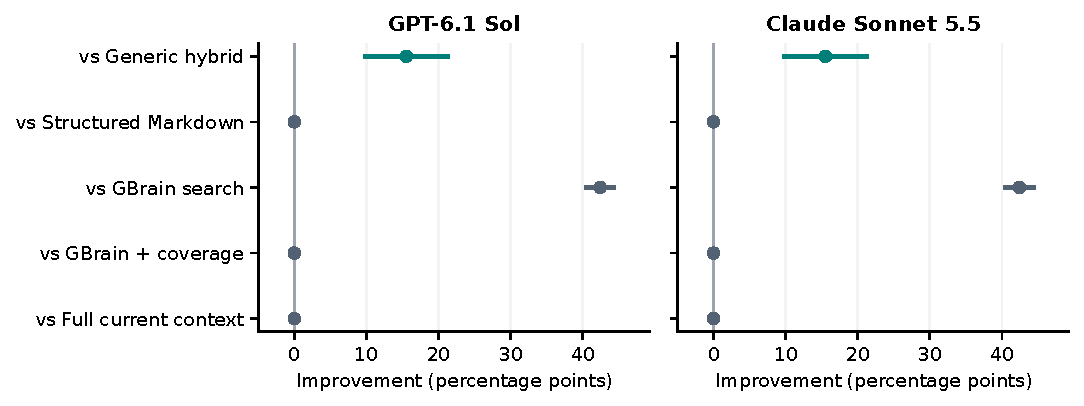
\includegraphics[width=\linewidth]{figures/integrated/paired-effects.pdf}
\caption{Paired Specialized-minus-comparator differences. The primary Generic contrast is highlighted; the other comparisons are descriptive. Zero differences against Markdown, GBrain+coverage and Full are observed ties, not formal equivalence tests.}
\label{fig:effects}
\end{figure}

\paragraph{The gain is recovered coverage, not reduced hallucination.}
Every arm withholds on all 132 negative cases per reader. No unsupported recommendation is observed. Generic's 41 missed positives and GBrain search's 112 missed positives per reader are abstentions where complete evidence was absent. Every positive packet with complete support produces a grounded action. The common validator changes no decision. No-context correctly withholds but covers none of the positive cases: its 50\% overall accuracy is an information-availability reference, not evidence of a weak model.

The qualitative audit selects the first Generic-failure/Specialized-success case in each family by sorted case ID. Missing seller geography blocks the partner and compliance cases; missing approved role, geography and offering pain block the renewal case. The same GPT correctly requests evidence, then recommends when coverage supplies those fields. Structured Markdown supplies them too. These traces localize the failure to evidence selection and show why a small general coverage mechanism can match specialization.

\begin{figure}[t]
\centering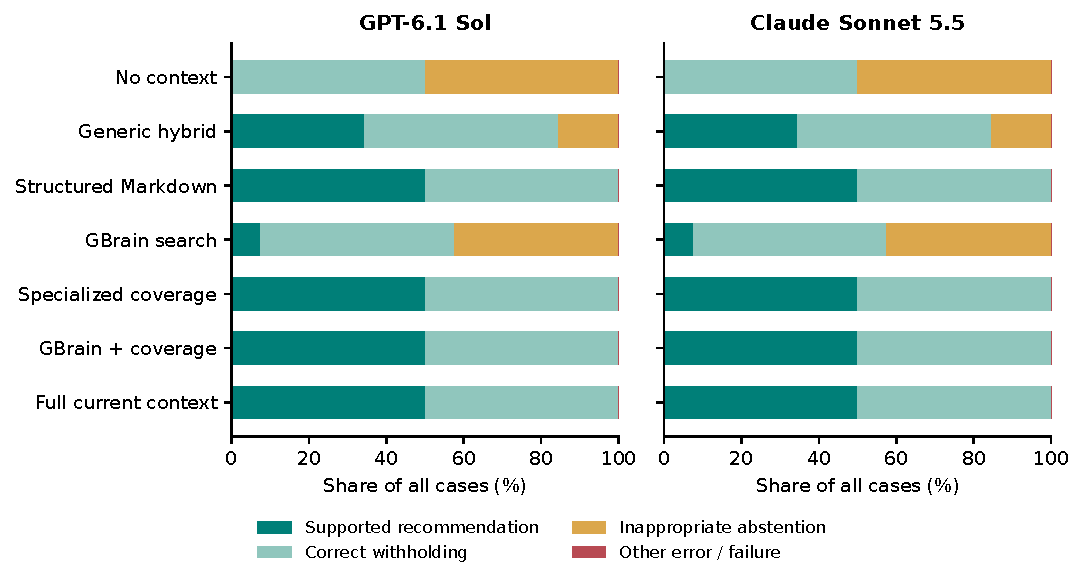
\includegraphics[width=\linewidth]{figures/integrated/decision-composition.pdf}
\caption{Outcome composition over all 264 cases per reader/arm. Supported recommendations and correct withholding are distinct. The remaining mass is inappropriate abstention on answerable cases; observed unsupported/error mass is zero.}
\label{fig:composition}
\end{figure}

\paragraph{Resources and action-interface checks.}
The main reader calls cost an estimated \$\MainCost{} from recorded usage. Specialized input averages 2,032 GPT tokens and 3,966 Claude tokens, versus 2,977 and 5,536 for Full: 31.7\% and 28.4\% less input with the same observed decisions. Total price also depends on output and cache behavior; it is not a pure measure of retrieval efficiency. Table~\ref{tab:resources} reports actual batch operating points. Cold local GBrain setup, source curation and production maintenance are not assigned invented dollar costs.

A separate post-hoc in-memory execution check completes all 1,278 proposed workflows through 2,606 mocked capability calls, with no external actions. It reads only supplied observations, verifies cited prerequisites and generates an evidence report within the declared allowance. This checks interface consistency; the scorer's simpler feasibility receipt is not mislabeled as execution, and neither check establishes campaign effectiveness.

The exact SQL reference solves all 264 cases from the permitted verified records without model calls. An LLM is therefore unnecessary for this formal eligibility problem once the facts and rules are clean; the comparison isolates evidence delivery to language-model readers, not a need for generative decision logic.
